\documentclass[10pt]{article}
\usepackage{epsfig}
\usepackage{graphicx}
\usepackage{amsmath}

% Fixme margin note package (turn on draft mode)
% \usepackage[final]{fixme}
% \usepackage[draft]{fixme}

\usepackage{color,listings}
\lstloadlanguages{APP}

\psfigdriver{dvips}

% New commands
\newcommand{\axx}{{\bf axx\ }}

\newcommand{\commentout}[1]{}

% change the title of the Fixme List
% \renewcommand{\listfixmename}{Things to Fix}

\newcommand{\comm}[2]{\bigskip
                      \begin{tabular}{|p{11cm}|}\hline
                      \multicolumn{1}{|c|}{{\bf Comment by #1}}\\ \hline
                      #2\\ \hline
                      \end{tabular}
                      \bigskip
                     }

\addtolength{\oddsidemargin}{-1.0in}
\addtolength{\evensidemargin}{-1.0in}
\addtolength{\textwidth}{2.0in}
\addtolength{\topmargin}{-0.5in}
\addtolength{\textheight}{1.5in}

% \pagenumbering{roman}
% \pagestyle{empty}
% \setcounter{page}{0}
% \thispagestyle{empty}

\sloppy

%---------------------------------------------------------------------
% Begin Document
%---------------------------------------------------------------------

\commentout{
   Outline for Talk

      Design of preprocessor
          AST
          Tree Traversal mechanism
          Queries
          Transformations

      Location of preprocessor

      Examples

 }

\begin{document}

\title{     A Brief Report on the Status of the  ROSE Project \\
              A Compiler Framework for the Optimization of \\ 
                    Object-Oriented Applications \\
                      How it works with Examples \\
                           (DRAFT DOCUMENT) } 

\author{Daniel J.\ Quinlan }
% {Center for Applied Scientific Computing\\
% Lawrence Livermore National Laboratory, Livermore, CA, USA\\
% }

\date{}

\maketitle

\tableofcontents

\pagenumbering{arabic}

\begin{abstract}
   ROSE is a compiler framework, it allow the development of specialized
preprocessors that address optimizations specific to a library's use within an application. For our
purposes in this talk, consider Kull to be the library and imagine a specialized preprocessor which
optimizes the use of Kull's abstractions within any C++ application.

   This talk introduces some results from the first non-trivial preprocessor developed using ROSE.
This preprocessor is intended to be both a working preprocessor useful for the Overture team and a
learning exercise for the ROSE team on the development of large scale preprocessors.  The examples I
will present are mostly from the optimization of the A++/P++ array class library, but the techniques
the use of ROSE would be the same for most of the abstractions found within the Kull Project.
\end{abstract}


\lstset{
 % language=C++,
   language=APP,
 % basicstyle=\small,                 % print whole listing small
   basicstyle=\scriptsize,            % print whole listing scriptsize
 % keywordstyle=\color{red}\bfseries\underbar, % underlined bold red keywords
 % keywordstyle=\bfseries\underbar, % underlined bold red keywords
   keywordstyle=\color{red}\bfseries, % underlined bold red keywords
   ndkeywordstyle=\color{blue}, % underlined bold red keywords
 % rdkeywordstyle=\color{blue}, % underlined bold red keywords
   identifierstyle={},                % nothing happens to other identifiers
 % identifierstyle=\color{blue},                % nothing happens to other identifiers
   commentstyle=\color{green},                % nothing happens to other identifiers
 % stringstyle=\ttfamily,             % typerwriter type for strings
 % stringstyle=\color{cyan}\ttfamily,             % typerwriter type for strings Magenta
   stringstyle=\color{magenta}\ttfamily,             % typerwriter type for strings Magenta
   stringspaces=false,                % no special string spaces
   labelstyle=\scriptsize,
   labelstep=1,
   labelsep=10pt
}

\section{Introduction}

   This talk on ROSE is meant to present examples of what ROSE can do and how it is currently used.
Current research work will of course simplify how ROSE will likely be used in the near future, but
even this work forms layers upon the current mechanism that will be demonstrated.  In this handout
I will present examples from the A++/P++ class library (part of the Overture Framework), but the examples
are only meant to demonstrate the use of a example abstraction.  Any similar abstraction could be
used, so my purpose is not to push the use of our array class libraries or Overture.

    The \axx preprocessor is an example of a preprocessor built using the ROSE compiler framework
and target the optimization of C++ applications using the A++\/P++ array class library.  The current
work only introduces serial transformations, parallel transformations will be introduced at a later
point.

    The A++\/P++ class library essentially represents the development of array abstractions in C++.
There are many serial array class libraries, but there are very few parallel array class libraries.
Applications developed using the A++ (serial) array class library can be recompiled to run in parallel
on distributed memory machines using the P++ (parallel) array class library.  The purpose of \axx is to
provide for optimizations that are not possible by the conventional C++ compiler.  \axx acts as a compiler,
but is really a source-to-source preprocessor that will call the back-end C++ compiler automatically (after
performing source-to-source transformations.  The generated code containing the transformations is not hidden
from the user and is placed in the same directory as the object file but with the prefix {\tt rose\_}.

\vspace{0.5in}

\begin{figure}[tb]
\begin{center}
\begin{tabular}{|c|} \hline
 Example Code \\\hline\hline
\begin{lstlisting}{}

  // Simple array statement
     A = 0;

  // Simple indexed array statement (using Index/Range objects)
     Range I,J;
     A(I,J) = B(I,J);

  // Simple 2D array stencil
     C(I,J) = C(I-1,J) + C(I+1,J) + C(I,J-1) + C(I,J+1);

  // Alternative scalar indexing version of simple 2D array stencil
     for (int j=0; j < D.getLength(1); j++)
          for (int i=0; i < D.getLength(0); i++)
               D(i,j) = D(i-1,j) + D(i+1,j) + D(i,j-1) + D(i,j+1);

\end{lstlisting}
\\\hline
\end{tabular}
\end{center}
\caption{ Example A++/P++ array statements. }
\label{AST_Code}
\end{figure}

% \newpage
\section{The Design of Preprocessors}

    The design of the \axx preprocessor follows the general design of all preprocessor built using
the ROSE compiler framework. We expect that a final version of \axx should be quite small, but at
present the implementation includes numerous features that will be moved into ROSE at some point.

\subsection{Abstract Syntax Tree (AST)}

     A general feature of the internal design of modern compilers is the representation of the
program as an abstract syntax tree (AST).  The AST is in general not really a tree, but a graph of
how pieces of the program are decomposed in terms of a languages grammar.  Figure \ref{AST_Graph}
shows and example AST for a trivial program shown in figure \ref{AST_Code}.

\begin{figure}[tb]
\begin{center}
\begin{tabular}{|c|} \hline
 Example Code \\\hline\hline
\begin{lstlisting}{}

int main() {
  int a[10];

  for(int i=0; i < 10; i++)
    a[i] = i * i;

  return 0;
}

\end{lstlisting}
\\\hline
\end{tabular}
\end{center}
\caption{ Example code used to generate AST. }
\label{AST_Code}
\end{figure}

\begin{figure}[tbh]
\begin{center}
\begin{tabular}{|c|} \hline
 Abstract Syntax Tree \\\hline\hline
\includegraphics[scale=0.9]{AST.ps}
\\\hline
\end{tabular}
\end{center}
\caption{AST representing example code. }
\label{AST_Graph}
\end{figure}

% \pagebreak


\subsection{Tree Traversal}

    A key piece of ROSE is the tree traversal mechanism, a collection of functions which take global
function pointers and execute the associated global functions on each of the nodes of the AST and
then call the respective traversal mechanism for all successor nodes.  In this way the global
functions are executed on all nodes of the AST in a predefined order.

% \begin{figure}[h]
% \begin{center}
% \begin{tabular}{|c|} \hline
%  Tree Traversal Interface \\\hline\hline
\begin{lstlisting}{}

// Class Definition
class TreeTraversal : public SgSimpleProcessing
   {
     public:
          void visit ( SgNode* astNode );
   };

// Source code appearing in ``main'' function
   TreeTraversal traversal;
   traversal.traverseInputFiles ( &sageProject, postorder );

\end{lstlisting}
% \\\hline
% \end{tabular}
% \end{center}
% \caption{ Tree Traversal Interface Example Code }
% \label{TreeTraversalInterfaceCode}
% \end{figure}


\subsection{Query Mechanism}

    The query mechanism is intimately associated with the tree traversal mechanism and represents
the interface of the tree traversal mechanism and the global functions that are executed on each
node.  Using approaches defined by attribute grammars, there are two different types of attributes:
inherited attributes and synthesized attributes.

% Within the current work we also add what we refer to as an {\em accumulator attribute}, but this is
% not a conventional feature of attribute grammars and may be removed.

\begin{itemize}
     \item {\bf Inherited Attributes} \\ Attributes represent values made available to
           subtrees. They are copied on each node from the parent to the child. If a parent modifies
           the inherited attribute it is see only by the children (and by recursion the whole
           subtree). These may be used as part of a pre-order or post-order traversal of the AST.

     \item {\bf Synthesized attributes} \\ Synthesized attributes are constructed from the child
           attributes on the way back up through the tree within the postorder tree traversal. Any
           possible synthesized attributes from children (successor nodes) are assembled into a
           single synthesized attribute and passed to parent nodes in the AST traversal (within the
           post-order traversal of the AST).

%    \item {\bf Accumulator attributes} \\ Attributes that are accessible from any point in the tree
%          traversal, essentially global variables made available to all nodes of the AST.
\end{itemize}

% \newpage
\subsection{Specification of Transformations}

    The \axx preprocessor uses the transformation specification mechanism defined within ROSE. These
mechanisms permit the specification of ascii text strings as a way to specify source code.  These
strings are assembled into intermediate program files internally and run through the front-end to
generate the AST fragments that the compiler understands.  Internally the compiler doesn't
understand strings, but only graphs (the AST), so the strings are converted to subgraphs.  The final
insertion/substitution of the transformation occurs as editing of the graph representing the AST.

A simple set of member functions at each node of the AST permit the editing of the AST using ascii strings to
specify new code to be generated.  Since any new code generated for use internally to edit the AST must be compiled to
generate an AST fragment, this process requires all local declarations and global declarations to compile properly.

AST editing functions available at each node of the AST include:
\begin{itemize}
    \item {\tt {\bf appendSourceCode} ( SgProject* project, string sourceCode, 
                             string localDeclarations, string globalDeclarations, bool isADeclaration);}
    \item {\tt {\bf prependSourceCode} ( SgProject* project, string sourceCode, 
                             string localDeclarations, string globalDeclarations, bool isADeclaration);}
    \item {\tt {\bf replaceSourceCode} ( SgProject* project, string sourceCode, 
                             string localDeclarations, string globalDeclarations, bool isADeclaration);}
    \item {\tt {\bf insertSourceCode} ( SgProject* project, string sourceCode, 
                             string localDeclarations, string globalDeclarations, bool locateNewCodeAtTop, bool isADeclaration);}
\end{itemize}

   In these member functions, the SgProject object contains the list of files to be processed and
information such as the input commandline which is reused for compiling intermediate generated files
(to generate AST fragments).  The {\tt string} objects represent the ascii source code associated with the
transformation's source code, and its supporting local declarations and global declarations.  Global declarations
include the ``\#include'' declarations required to read head all header files required for compiling the transformation.

The following code shows an example of an intermediate file generated internally.  This file is compiled using the 
commandline arguments input to \axx (the same commandline that the user has specified for compiling his application).
The AST generated from the compilation of this intermediate file is processed internally to extract out its relevant parts.
The AST fragments extracted are then inserted into the application program's AST using the AST editing functions presented in 
previously.

\commentout{
   The following example file is internally generated and is never seen by the user (though it is
not deleted by the preprocessor phases). It is assembled from the source code strings input to the
AST editing functions.

\vspace{0.5in}

\begin{lstlisting}{}

// ################################################################
// THIS IS AN AUTOMATICALLY GENERATED FILE (DO NOT EDIT THIS FILE!)
// ################################################################

#include "simpleA++.h" 
#define ROSE_MACROS_APPEAR_AS_FUNCTIONS 
#include "transformationMacros.h" 

// Variables used in this transformation (automatically generated from simple dependence analysis of original code before transformation) 
Range I; 
Range J; 
double Mesh_Size; 
doubleArray Right_Hand_Side; 
doubleArray Solution; 


doubleArray _T;int SC_Right_Hand_Side_I_J(int,int); int SC_Solution_I_J(int,int); int SC__T_I_J(int,int); int _Right_Hand_Side; int _Right_Hand_Side_I_J; int _Solution; int _Solution_I_J; int __T; int __T_I_J; 

int
transformationContainerFunction() 
   {
          // Automatically Introduced Transformation (via preprocessor built by ROSE)
          // { 
          // These loop index declarations could later be declared just once in the same scope as the statement being transformed 
          int VARIABLE_DECLARATIONS_MARKER_START; 
             ARRAY_OPERAND_VARIABLE_SIZE_DECLARATION_MACRO_D2(_Right_Hand_Side);
             ARRAY_OPERAND_VARIABLE_SIZE_DECLARATION_MACRO_D2(_Solution);
             ARRAY_OPERAND_VARIABLE_SIZE_DECLARATION_MACRO_D2(__T);
             double* APP_RESTRICT _Right_Hand_Side_I_J_pointer = NULL;
             double* APP_RESTRICT _Solution_I_J_pointer = NULL;
             double* APP_RESTRICT __T_I_J_pointer = NULL;
          ARRAY_OPERAND_VARIABLE_STRIDE_DECLARATION_MACRO_D2(_Right_Hand_Side_I_J);
          ARRAY_OPERAND_VARIABLE_STRIDE_DECLARATION_MACRO_D2(_Solution_I_J);
          ARRAY_OPERAND_VARIABLE_STRIDE_DECLARATION_MACRO_D2(__T_I_J);
          LOOP_INDEX_VARIABLES_DECLARATION_MACRO_D2();
           
          int VARIABLE_DECLARATIONS_MARKER_END; 
          int VARIABLE_INITIALIZATION_MARKER_START; 
          // undef subscript computation macro (before transformation) 
           
             "ROSE-TRANSFORMATION-MACRO:#define SC_Right_Hand_Side_I_J(x1,x2) /* case VariableSizeVariableStride */ \                  (x1)*_Right_Hand_Side_I_J_stride1+((x2)*_Right_Hand_Side_I_J_stride2*_Right_Hand_Side_size1)"; 
             "ROSE-TRANSFORMATION-MACRO:#define SC_Solution_I_J(x1,x2) /* case VariableSizeVariableStride */ \
                  (x1)*_Solution_I_J_stride1+((x2)*_Solution_I_J_stride2*_Solution_size1)"; 
             "ROSE-TRANSFORMATION-MACRO:#define SC__T_I_J(x1,x2) /* case VariableSizeVariableStride */ \
                  (x1)*__T_I_J_stride1+((x2)*__T_I_J_stride2*__T_size1)"; 
             ARRAY_OPERAND_VARIABLE_SIZE_INITIALIZATION_MACRO_D2(Right_Hand_Side,_Right_Hand_Side);
             ARRAY_OPERAND_VARIABLE_SIZE_INITIALIZATION_MACRO_D2(Solution,_Solution);
             ARRAY_OPERAND_VARIABLE_SIZE_INITIALIZATION_MACRO_D2(_T,__T);
             _Right_Hand_Side_I_J_pointer = Right_Hand_Side.getAdjustedDataPointer(I,J); 
             _Solution_I_J_pointer = Solution.getAdjustedDataPointer(I,J); 
             __T_I_J_pointer = _T.getAdjustedDataPointer(I,J); 
          ARRAY_OPERAND_VARIABLE_STRIDE_INITIALIZATION_MACRO_D2(Right_Hand_Side,_Right_Hand_Side_I_J);
          ARRAY_OPERAND_VARIABLE_STRIDE_INITIALIZATION_MACRO_D2(Solution,_Solution_I_J);
          ARRAY_OPERAND_VARIABLE_STRIDE_INITIALIZATION_MACRO_D2(_T,__T_I_J);
          ARRAY_TRANSFORMATION_LENGTH_INITIALIZATION_MACRO_D2(Solution);
           
          int VARIABLE_INITIALIZATION_MARKER_END; 
          int TRANSFORMATION_MARKER_START; 
          _T.redim(Solution);
          // "for" loop for $dimD array operations with stride 
             for (_2 = 0; _2 < _length2; _2++) { 
             for (_1 = 0; _1 < _length1; _1++) { 
                __T_I_J_pointer[SC__T_I_J(_1,_2)] = 
                     ((((((((((Mesh_Size*Mesh_Size*
                     _Right_Hand_Side_I_J_pointer[SC_Right_Hand_Side_I_J(_1,_2)])+
                     _Solution_I_J_pointer[SC_Solution_I_J((_1+1),_2)])+
                     _Solution_I_J_pointer[SC_Solution_I_J((_1-1),_2)])+
                     _Solution_I_J_pointer[SC_Solution_I_J(_1,(_2+1))])+
                     _Solution_I_J_pointer[SC_Solution_I_J(_1,(_2-1))])+
                     _Solution_I_J_pointer[SC_Solution_I_J((_1+1),(_2+1))])+
                     _Solution_I_J_pointer[SC_Solution_I_J((_1+1),(_2-1))])+
                     _Solution_I_J_pointer[SC_Solution_I_J((_1-1),(_2+1))])+
                     _Solution_I_J_pointer[SC_Solution_I_J((_1-1),(_2-1))])/8.0); 
                } 
                } 
          // "for" loop for $dimD array operations with stride 
             for (_2 = 0; _2 < _length2; _2++) { 
             for (_1 = 0; _1 < _length1; _1++) { 
                _Solution_I_J_pointer[SC_Solution_I_J(_1,_2)] = __T_I_J_pointer[SC__T_I_J(_1,_2)]; 
                } 
                } 
           
          int TRANSFORMATION_MARKER_END; 
          // }
           
     return 0;
   }

\end{lstlisting}
}

\subsection{Example Preprocessor: Instrumentation}

   This example preprocessor is a complete compiler which takes in a C++ source code and outputs and
object file (or executable) just like any other compiler.  In this case the goal of the
transformations are to instrument the code.  The instrumentation consists of adding a function call,
to {\tt myTimerFunctionStart()}, to a top of each block (scope) and a function call, to {\tt
myTimerFunctionEnd()}, to the bottom of each block (scope).  

\commentout{
In order to be completely
self-contained, and additional transformation inserts the definitions of {\tt
myTimerFunctionStart()} and {\tt myTimerFunctionEnd()} at the top of the program (just before the
{\tt main()} function).
}

   The definitions of the functions and the function call statements consist of ascii strings and
are inserted into the AST using the AST method functions {\tt prependSourceCode} and {\tt
insertSourceCode}.  This simplified approach to the editing of the AST is a new and novel feature of
the ROSE compiler framework (it is not done by any other compiler that I'm aware of) and is an
example of how we simplify the specification of transformations to make them accessible to library
developers and others without an extensive compiler background.

\vspace{0.5in}

\begin{lstlisting}{}

// ROSE is a tool for building preprocessors, this file is an example preprocessor built with ROSE.
// Specifically it shows the design of a transformation to instrument source code, placing source code
// at the top and bottom of each basic block.

#ifdef HAVE_CONFIG_H
#include <config.h>
#endif

#include "rose.h"
#include "Cxx_GrammarTreeTraversalClass.h"

class SimpleInstrumentation : public SgSimpleProcessing
   {
     public:
          void visit ( SgNode* astNode );
   };

void
SimpleInstrumentation::visit ( SgNode* astNode )
   {
     if (astNode->variantT() == V_SgBasicBlock)
        {
          const int SIZE_OF_BLOCK = 2;
          if (isSgBasicBlock(astNode)->get_statements().size() >= SIZE_OF_BLOCK)
             {
               string globalDeclarations = "void myTimerFunctionStart(); void myTimerFunctionEnd();";
               string codeAtTopOfBlock    = "myTimerFunctionStart();";
               string codeAtBottomOfBlock = "myTimerFunctionEnd();";

            // Build a new AST fragment and insert it into the AST
               bool locateNewCodeAtTop = true;
               bool isADeclaration = true;
               astNode->insertSourceCode(*globalProject,codeAtTopOfBlock,localDeclarations,
                                          globalDeclarations,locateNewCodeAtTop,isADeclaration);
               locateNewCodeAtTop = false;
               astNode->insertSourceCode(*globalProject,codeAtBottomOfBlock,localDeclarations,
                                         globalDeclarations,locateNewCodeAtTop,isADeclaration);
             }
        }
   }

int
main ( int argc, char * argv[] )
   {
  // Build the project object which we will fill up with multiple files and use as a
  // handle for all processing of the AST(s) associated with one or more source files.
     int EDG_FrontEndErrorCode = 0;
     SgProject sageProject (argc,argv,EDG_FrontEndErrorCode);

  // Traverse the AST and do queries and/or transformations
     SimpleInstrumentation treeTraversal;
     treeTraversal.traverseInputFiles ( &sageProject );

  // Generate the final C++ source code from the potentially modified SAGE AST
     sageProject.unparse();

  // What remains is to run the specified compiler (typically the C++ compiler) using 
  // the generated output file (unparsed and transformed application code) to generate
  // an object file.
     int finalCombinedExitStatus = sageProject.compileOutput();

  // return any errors generated by the backend compilation of the modified source code
     return finalCombinedExitStatus;
   }

\end{lstlisting}

\vspace{0.5in}

   Running the instrumentation preprocessor on the following example code:

\begin{lstlisting}{}

int
main ( int argc, char * argv[] )
   {
     int boolean;
     int n = 100;
     if (boolean)
        {
          int x;
          int y;
	  for (int i=0; i < n; i++)
	     {
               int x;
               int y;
	     }
        }
       else
        {
          int y;
          int z;
        }
     
     return 0;
   }

\end{lstlisting}

\vspace{0.5in}

generates the instrumented code show below:

\begin{lstlisting}{}

int main(int argc,char * * argv)
   { 
     myTimerFunctionStart();
     int boolean; 
     int n = 100; 
     if (boolean)
        { 
          myTimerFunctionStart();
          int x; 
          int y; 
          for (int i = 0; i < n; i++)
             { 
               myTimerFunctionStart();
               int x; 
               int y; 
               myTimerFunctionEnd(); 
             } 
          myTimerFunctionEnd(); 
        } 
       else
        { 
          myTimerFunctionStart();
          int y; 
          int z; 
          myTimerFunctionEnd(); 
        } 
     myTimerFunctionEnd();
     return 0;
  }

\end{lstlisting}


\section{A Tour of Code from the \axx Preprocessor}

   A more complex example showing a more sophisticated use of ROSE is in the implementation
of the \axx preprocessor.  We show two of the functions from the implementation of \axx.
These examples show the use of the inherited, synthesized, and accumulator attributes.

   The \axx will eventually have many different transformations, the design presently contains an
array transformation mechanism which was only one transformation implemented; the {\bf {\it array
assignment statement transformation}}. Additional transformations will be added and include:

\begin{itemize}
     \item {\bf Scalar Indexing Transformation} \\ Used to optimize the use of scalar indexing of
     A++\/P++ array objects where possible.

     \item {\bf Parallel Message Scheduling Transformations} \\ The generation of MPI calls can be
     moved/aggregated to optimize parallel communication.
\end{itemize}

   Within the {\it array assignment statement transformation} within the \axx preprocessor we use all three forms of attributes.
\begin{itemize}
     \item {\bf Inherited Attributes} \\ Used to communicate if array operand are indexed.  If they
           are indexed then it is set in the inherited attribute so that it can be read in the
           assemble function on the way back up the tree.  This communicates to the processing of
           the variable reference case within the assembly function that it does not have to
           complete the substring processing (since it will be completed by the processing of the
           index arguments later).

     \item {\bf Synthesized attributes} \\ Synthesized attributes are used to carry the assemble
           pieces of the transformation back up the tree (the transformations are separated into
           declarations, initializations, and the specification).  This is a part of the post-order
           traversal of the tree.

%    \item {\bf Accumulator attributes} \\ An accumulator attribute is used (referenced on each
%          node, essentially like a global variable) to hold the operand data base which stores the
%          names of the operands and an index database for each operand (containing the names of the
%          index objects used for that operand).
\end{itemize}

The following sections present the example code used within the local function and assembly function
to generate and manipulate these attributes.

\subsubsection{Scalar Indexing Statement Transformation}

   This is the simpler of two transformations presently implemented in \axx.  The transformation
takes code of the form shown in figure \ref{UnoptimizedScalarIndexingExample} and transforms it into
code of the form in figure \ref{ROSETransformedScalarIndexingExample}.  The point of the
transformation is to address the 30\% to 400\% performance degradation associated with scalar
indexing of array objects.  The issue is not specific to A++/P++, but has to do with the subscript
computation requiring access to the data members of the array object and the general lack of
optimization associated with data fields of a structure (or class in this case) by the compiler.
The performance improvement associated with this transformation is compiler dependent and also
depends upon the statement and the degree of generality of the subscript computation.

\begin{figure}[h]
\begin{center}
\begin{tabular}{|c|} \hline
 Example Code \\\hline\hline
\begin{lstlisting}{}

  // Scalar indexing version of simple 2D array stencil
     for (int j=0; j < D.getLength(0); j++)
          for (int i=0; i < D.getLength(0); i++)
               D(i,j) = D(i-1,j) + D(i+1,j) + D(i,j-1) + D(i,j+1);

\end{lstlisting}
\\\hline
\end{tabular}
\end{center}
\caption{ Example of scalar indexing of array object. }
\label{UnoptimizedScalarIndexingExample}
\end{figure}


\begin{figure}[h]
\begin{center}
\begin{tabular}{|c|} \hline
 Example Code \\\hline\hline
\begin{lstlisting}{}

  // Scalar indexing showing use of inlined functions
     for (int j=0; j < D.size[1]; j++)
          for (int i=0; i < D.size[0]; i++)
               D.data[i+j*D.size[0]] =
                    D.data[(i-1)+j*D.size[0]] + D.data[(i+1)+j*D.size[0]] +
                    D.data[i+(j-1)*D.size[0]] + D.data[i+(j+1)*D.size[0]];

\end{lstlisting}
\\\hline
\end{tabular}
\end{center}
\caption{ Example of scalar indexing showing use of inlined functions (after inlining). }
\label{InlinedScalarIndexingExample}
\end{figure}

   Figure \ref{InlinedScalarIndexingExample} shows the effect of inlining and the essential problem that
the compiler can't adequately resolve in the optimization.  Specifically the subscript computation is
expressed in terms of field values of the array object (date member of the array object).  The compiler
can't see to optimize this further because the value of D.data could point to and of the data members
(even though we know this is ridiculous, this is an example of the semantics that is not known to the
compiler).

\begin{figure}[h]
\begin{center}
\begin{tabular}{|c|} \hline
 Example Code \\\hline\hline
\begin{lstlisting}{}

  // Scalar indexing showing transformation
     double* Dptr = D.data;
     int size0 = D.size[0];
     int size1 = D.size[1];
     for (int j=0; j < size1; j++)
          for (int i=0; i < size0; i++)
               Dptr[i+j*size] =
                    Dptr[(i-1)+j*size0] + Dptr[(i+1)+j*size0] +
                    Dptr[i+(j-1)*size0] + Dptr[i+(j+1)*size0];

\end{lstlisting}
\\\hline
\end{tabular}
\end{center}
\caption{ Example of scalar indexing transformation. }
\label{TransformedScalarIndexingExample}
\end{figure}

\begin{figure}[h]
\begin{center}
\begin{tabular}{|c|} \hline
 Example Code \\\hline\hline
\begin{lstlisting}{}

  // Scalar indexing showing transformation
     double* restrict Dptr = D.data;
     int size0 = D.size[0];
     int size1 = D.size[1];
     for (int j=0; j < size1; j++)
          for (int i=0; i < size0; i++)
#define SC(x1,x2) (x1)+(x2*size0)
               D_pointer[SC(i,j)] =
                    D_pointer[SC(i-1,j)] + D_pointer[SC(i+1,j)] +
                    D_pointer[SC(i,j-1)] + D_pointer[SC(i,j+1)];
#undef SC

\end{lstlisting}
\\\hline
\end{tabular}
\end{center}
\caption{ Example of scalar indexing showing code generated by \axx (still incomplete). }
\label{ROSETransformedScalarIndexingExample}
\end{figure}

   Figure \ref{TransformedScalarIndexingExample} shows the code that we might want to be generated instead of
the inlined code in figure \ref{InlinedScalarIndexingExample}.  The difference in performance between these is 
30\% to 400\% depending upon the compiler (always with full optimizations applied).  The code generated
by the \axx preprocessor in figure \ref{ROSETransformedScalarIndexingExample} is equivaliant to that of 
the optimizing transformation in figure \ref{TransformedScalarIndexingExample}, but with the subscript 
computation expressed through macro.



\subsubsection{Synthesized Attribute Assembly function from Scalar Indexing Statement Transformation}

The assembly function takes attributes generated by the local function and generates from child
synthesized attributes a single synthesized attribute (hence the name {\bf synthesized attribute}).

\vspace{0.5in}

{\scriptsize
\begin{lstlisting}{}

ScalarIndexingStatementQuerySynthesizedAttributeType
ScalarIndexingStatementTransformation::
evaluateSynthesizedAttribute (
   SgNode* astNode,
   ScalarIndexingStatementQueryInheritedAttributeType ScalarIndexingStatementQueryInheritedData,
   SubTreeSynthesizedAttributes synthesizedAttributeList )
   {
     ScalarIndexingStatementQuerySynthesizedAttributeType returnSynthesizedAttribute (synthesizedAttributeList);

  // Build up a return string
     string returnString;

  // Need to handle all unary and binary operators and variables (but not much else)
     switch (astNode->variant())
        {
       // Handle binary operators
          case ADD_OP:
          case SUBT_OP:
          case MULT_OP:
          case DIV_OP:
          case INTEGER_DIV_OP:
          case MOD_OP:
          case AND_OP:
          case OR_OP:
          case BITXOR_OP:
          case BITAND_OP:
          case BITOR_OP:
          case EQ_OP:
          case LT_OP:
          case GT_OP:
          case NE_OP:
          case LE_OP:
          case GE_OP:
          case ASSIGN_OP:
          case BINARY_EXPRESSION:
             {
               string operatorString = TransformationSupport::buildOperatorString (astNode);
               returnString = synthesizedAttributeList[SgBinaryOp_lhs_operand_i].getTransformationString() +
                              operatorString +
                              synthesizedAttributeList[SgBinaryOp_rhs_operand_i].getTransformationString();
               returnSynthesizedAttribute.setTransformationString(returnString);
               break;
             }

       // Handle case function paramter list
          case EXPR_LIST:
             {
               returnString = astNode->unparseToString();
               returnSynthesizedAttribute.setTransformationString(returnString);
               break;
             }

       // Case for array::operator()
          case FUNC_CALL: // tag for SgFunctionCallExp class
             {
               SgFunctionCallExp* functionCallExpression = isSgFunctionCallExp(astNode);
               string operatorName     = TransformationSupport::getFunctionName ( functionCallExpression );
               string functionTypeName = TransformationSupport::getFunctionTypeName(functionCallExpression);

               if ( (functionTypeName == "doubleArray") ||
                    (functionTypeName == "floatArray")  ||
                    (functionTypeName == "intArray") )
                  {
                    SgExprListExp* exprListExp              = functionCallExpression->get_args();
                    SgExpressionPtrList & expressionPtrList = exprListExp->get_expressions();
                    int numberOfParameters = expressionPtrList.size();

                    TransformationSupport::operatorCodeType operatorCodeVariant =
                         TransformationSupport::classifyOverloadedOperator (operatorName.c_str(),numberOfParameters);

                 // Separating this case into additional cases makes up for using a more
                 // specific higher level grammar (which is not finished yet).
                    if ( operatorCodeVariant == TransformationSupport::PARENTHESIS_OPERATOR_CODE)
                       {
                         ROSE_ASSERT (operatorName == "operator()");

                      // Now get the operands out and search for the offsets in the index objects
                         list<int> & transformationOptionList =
                              ScalarIndexingStatementQueryInheritedData.getTransformationOptions();

                         string operandIdentifier  =
                            synthesizedAttributeList[SgFunctionCallExp_function].getTransformationString();
                         string argumentListString =
                            synthesizedAttributeList[SgFunctionCallExp_args].getTransformationString();

                      // gather variable name data for later generation of subscript macro and supporting declarations
                         accumulatorValue.operandDataBase.setVariableName(operandIdentifier);

                         returnString = operandIdentifier + "_pointer[SC(" + argumentListString + ")]";
                       }
                  }

               returnSynthesizedAttribute.setTransformationString(returnString);
               break;
             }

       // Handle values
          case ValueExpTag:
          case BOOL_VAL:
          case STRING_VAL:
          case SHORT_VAL:
          case CHAR_VAL:
          case UNSIGNED_CHAR_VAL:
          case WCHAR_VAL:
          case UNSIGNED_SHORT_VAL:
          case ENUM_VAL:
          case UNSIGNED_INT_VAL:
          case LONG_INT_VAL:
          case LONG_LONG_INT_VAL:
          case UNSIGNED_LONG_LONG_INT_VAL:
          case UNSIGNED_LONG_INT_VAL:
          case INT_VAL:
          case FLOAT_VAL:
          case DOUBLE_VAL:
          case LONG_DOUBLE_VAL:
             {
               string returnString = astNode->unparseToString();
               returnSynthesizedAttribute.setTransformationString(returnString);
               break;
             }

          case VAR_REF:
             {
            // A VAR_REF has to output a string (the variable name)
               SgVarRefExp* varRefExp = isSgVarRefExp(astNode);
               SgVariableSymbol* variableSymbol = varRefExp->get_symbol();
               string variableName = variableSymbol->get_declaration()->get_name().str();
               returnSynthesizedAttribute.setTransformationString(variableName);
               break;
             }

          default:
             {
               SubTreeSynthesizedAttributes::iterator i;
               for (i = synthesizedAttributeList.begin(); i != synthesizedAttributeList.end(); i++)
                  {
                    returnSynthesizedAttribute += *i;
                  }
               break;
             }
        }

     return returnSynthesizedAttribute;
   }

\end{lstlisting}
}


% \newpage
\section{How to Control Optimizations within \axx}
    By default all transformation generate completely general code (though currently we exclude
indirect addressing and where statement transformations).  The user can control optimizations within
the preprocessor through the declaration of variables of a specific type (TransformationAssertion
objects) and the input of specific options to their constructors.

Options that can be used at parameters to control the preprocessor optimizations include:
\begin{itemize}
   \item SkipTransformation             (not implemented)
   \item NoWhereStatementTransformation (not implemented)
   \item WhereStatementTransformation   (not implemented)
   \item NoIndirectAddressing           (not implemented)
   \item IndirectAddressing             (not implemented)
   \item ConstantStrideAccess
   \item StrideOneAccess
   \item VariableStrideAccess
   \item SameSizeArrays
   \item DifferentSizeArrays
   \item SameParallelDistributions      (not implemented)
   \item DifferentParallelDistributions (not implemented)
\end{itemize}

   Since the mechanism uses variable declarations as a way to control the optimization, the syntax is:
   $$ TransformationAssertion <unique variable name> (<option>); $$

   The following example shows addition of declarations to the global, local scopes to control of
optimizations by the preprocessor:

\vspace{0.5in}

\begin{lstlisting}{}

#include ``A++.h''

// Mechanism to specify options to the preprocessor (global scope)
// Currently we don't handle where statements or indirect addressing (so assert that there are none)
TransformationAssertion globalScope0 (TransformationAssertion::NoWhereStatementTransformation,
                                      TransformationAssertion::NoIndirectAddressing);

int main()
   {
  // First optimization permits all the size# variables to be the same across all operands (this
  // should significantly reduce the register pressure).
     TransformationAssertion assertion1 (TransformationAssertion::SameSizeArrays);

  // Specification of uniform stride permits all the <name>_stride# variables to be the same across
  // all operands (further reducing the register pressure).
     TransformationAssertion assertion2 (TransformationAssertion::ConstantStrideAccess);

     bool booleanValue = TRUE;
     doubleArray A(10);
     doubleArray B(10);

     A = 0;
     B = 0;

     if (booleanValue)
        {
       // In addition to uniform stride we specify here that the stride is lenght 1 which permits
       // additional optimizations to the subscript computation (or the loop nest) to remove the stride
       // variable from the computations altogether.
          TransformationAssertion assertion3 (TransformationAssertion::StrideOneAccess);

       // stride 1 array statements
          Range I (1,8,1);
          A(I) = ( A(I-1) + A(I+1) ) * 0.5;
        }
       else
        {
       // Turn off the same size array optimizations (generate size variables for each operand)
          TransformationAssertion assertion3 (TransformationAssertion::DifferentSizeArrays);

       // Turn off the unit and uniform stride optimizations (generate stride variables for each operand)
          TransformationAssertion assertion4 (TransformationAssertion::VariableStrideAccess);

       // stride 2 array statements
          Range I (1,8,2);
          Range J (1,8,1);
          A(J) = ( B(I-1) + B(I+1) ) * 0.5;
        }

     return 0;
   }

\end{lstlisting}

% \newpage
\section{Examples}
    This section presents numerous examples of transformations that are automated using \axx.

\subsection{Simple Assignment Statement}

\subsubsection{Default transformation without specification of semantic assertions}

    If the mechanism for specifying the semantics in the users application is {\bf NOT} used then we
can't currently know that the array operands have the same size, stride, or know anything specific
about the values associated with the strides (e.g. stride 1 access).  In this case the
transformations are generated with a degree of generality that allows them to be executed
independent their context within the application.  The trade-off is that the transformation will
have additional overhead which might otherwise be optimized away.


   The following trivial example shows an array statement.  In this case a single expression is represented
(the doubleArray::operator=()).

   For the array statement:
\vspace{0.5in}

\begin{lstlisting}{}

doubleArray A(10);
A = 0;

\end{lstlisting}

% \newpage

   we generate the following transformation:

\vspace{0.5in}

\begin{lstlisting}{}

int functionA()
   { 
     ARRAY_OPERAND_VARIABLE_SIZE_DECLARATION_MACRO_D6(_A); 
     double * _A_pointer = ((double * )0); 
     ARRAY_OPERAND_VARIABLE_STRIDE_DECLARATION_MACRO_D6(_A); 
     int _1; 
     int _2; 
     int _3; 
     int _4; 
     int _5; 
     int _6; 
     int _length1 = 0; 
     int _length2 = 0; 
     int _length3 = 0; 
     int _length4 = 0; 
     int _length5 = 0; 
     int _length6 = 0;
     class doubleArray A(10);
     ARRAY_OPERAND_VARIABLE_SIZE_INITIALIZATION_MACRO_D6(A,_A); 
     ARRAY_OPERAND_VARIABLE_STRIDE_INITIALIZATION_MACRO_D6(A,_A); 
     ARRAY_TRANSFORMATION_LENGTH_INITIALIZATION_MACRO_D6(A); 
     _A_pointer = (A.getAdjustedDataPointer)(); 
     #define SC_A(x1,x2,x3,x4,x5,x6) /* case VariableSizeVariableStride */ \
          (x1)*_A_stride1+((x2)*_A_stride2*_A_size1)+((x3)*_A_stride3*_A_size2)+\
         ((x4)*_A_stride4*_A_size3)+((x5)*_A_stride5*_A_size4)+((x6)*_A_stride6*_A_size5)
; 
     for (_6 = 0; _6 < _length6; _6++)
        { 
          for (_5 = 0; _5 < _length5; _5++)
          { 
            for (_4 = 0; _4 < _length4; _4++)
            { 
              for (_3 = 0; _3 < _length3; _3++)
              { 
                for (_2 = 0; _2 < _length2; _2++)
                { 
                  for (_1 = 0; _1 < _length1; _1++)
                  { 
                    _A_pointer[SC_A(_1,_2,_3,_4,_5,_6)] = 0.0; 
                  } 
                } 
              } 
            } 
          } 
        } 

     return 0;
} 

\end{lstlisting}

Within this case, because we didn't know the dimensionality of the array object {\tt A}, we were
forced to assume it could have the maximal dimensionality representable in the A++/P++ array class
library.  The semantics of array objects is that they can be up to six dimensional.  So the
transformation requires a six level loop next to be generated.  Notice also that subscript
computation represented by the macro {\tt SC\_A(x1,x2,x3,x4,x5,x6)} is six dimensional and contains
variables representing the stride (e.g. {\tt \_A\_stride6}) and the size (e.g. {\tt \_A\_size5}).

If we were to know at compile time that the stride have the value 1, then the stride variables could
have been eliminated from the subscript computation.  The resulting code would have fewer variables
associated with its subscript computation and, in the case of statements involving several operands,
would be more efficient.

\subsubsection{Specification of Transformation Assertions (assert stride == 1)}

   The following code shows the transformation for the case of where the user has specified directly in his
code that the stride has the value one (stride == 1).

\vspace{0.5in}

\begin{lstlisting}{}

int functionE()
   { 
     ARRAY_OPERAND_VARIABLE_SIZE_DECLARATION_MACRO_D6(_A); 
     double * _A_pointer = ((double * )0); 
     int _1; 
     int _2; 
     int _3; 
     int _4; 
     int _5; 
     int _6; 
     int _length1 = 0; 
     int _length2 = 0; 
     int _length3 = 0; 
     int _length4 = 0; 
     int _length5 = 0; 
     int _length6 = 0; 

  // Specify unit stride to generate better optimized execution (removes stride from computation)
     class TransformationAssertion assertion3(TransformationAssertion::StrideOneAccess); 

     class doubleArray A(10);
     ARRAY_OPERAND_VARIABLE_SIZE_INITIALIZATION_MACRO_D6(A,_A); 
     ARRAY_TRANSFORMATION_LENGTH_INITIALIZATION_MACRO_D6(A); 
     _A_pointer = (A.getAdjustedDataPointer)(); 
     #define SC_A(x1,x2,x3,x4,x5,x6) /* case VariableSizeUnitStride */ \
          (x1)+((x2)*_A_size1)+((x3)*_A_size2)+((x4)*_A_size3)+((x5)*_A_size4)+((x6)*_A_size5)
; 
     for (_6 = 0; _6 < _length6; _6++)
        { 
          for (_5 = 0; _5 < _length5; _5++)
          { 
            for (_4 = 0; _4 < _length4; _4++)
            { 
              for (_3 = 0; _3 < _length3; _3++)
              { 
                for (_2 = 0; _2 < _length2; _2++)
                { 
                  for (_1 = 0; _1 < _length1; _1++)
                  { 
                    _A_pointer[SC_A(_1,_2,_3,_4,_5,_6)] = 0.0; 
                  } 
                } 
              } 
            } 
          } 
        } 

     return 0;
   } 

\end{lstlisting}

% \newpage
\subsection{More interesting array statements: Residual Computation}

   The following array statement has more operands, includes indexing, and shows a generally
more complex array statement and the transformations that are generated with different explicit
transformation assertions added to the user's original source code.

% \subsubsection{Single Statements with no Loop Dependence}

   Stencils are interesting because they occur often in scientific computing.

\subsubsection{Initial array statement before transformation}

   This shows the A++\/P++ array statement before transformation:

\vspace{0.5in}

\begin{lstlisting}{}
     int n; \
     Range I,J,K; \
     doubleArray Residual(n,n,n); \
     doubleArray Right_Hand_Side(n,n,n); \
     doubleArray Solution(n,n,n); \
     double Scaling_Factor; \
     Residual (I,J,K) = Right_Hand_Side (I,J,K) + Scaling_Factor * ( \
                        Solution (I+1,J,K) + Solution (I-1,J,K) + \
                        Solution (I,J-1,K) + Solution (I,J+1,K) + Solution (I,J,K-1) + \
                        Solution (I,J,K+1) - 6.0 * Solution (I,J,K) );
\end{lstlisting}

% \newpage

\subsubsection{Default transformation with no transformation assertions}

The following transformation assumes no user specified transformation assertions (see previous sections):

\begin{lstlisting}{}
int functionA()
   { 
     ARRAY_OPERAND_VARIABLE_SIZE_DECLARATION_MACRO_D3(_Residual); 
     ARRAY_OPERAND_VARIABLE_SIZE_DECLARATION_MACRO_D3(_Right_Hand_Side); 
     ARRAY_OPERAND_VARIABLE_SIZE_DECLARATION_MACRO_D3(_Solution); 
     double * _Residual_I_J_K_pointer = ((double * )0); 
     double * _Right_Hand_Side_I_J_K_pointer = ((double * )0); 
     double * _Solution_I_J_K_pointer = ((double * )0); 
     ARRAY_OPERAND_VARIABLE_STRIDE_DECLARATION_MACRO_D3(_Residual_I_J_K); 
     ARRAY_OPERAND_VARIABLE_STRIDE_DECLARATION_MACRO_D3(_Right_Hand_Side_I_J_K); 
     ARRAY_OPERAND_VARIABLE_STRIDE_DECLARATION_MACRO_D3(_Solution_I_J_K); 
     int _1; 
     int _2; 
     int _3; 
     int _length1 = 0; 
     int _length2 = 0; 
     int _length3 = 0;
     int n;
     class Range I; 
     class Range J;
     class Range K;
     class doubleArray Residual(n,n,n);
     class doubleArray Right_Hand_Side(n,n,n);
     class doubleArray Solution(n,n,n);
     double Scaling_Factor; 
     #define SC_Residual_I_J_K(x1,x2,x3) /* case VariableSizeVariableStride */ \
          (x1)*_Residual_I_J_K_stride1+((x2)*_Residual_I_J_K_stride2*_Residual_size1)+\
         ((x3)*_Residual_I_J_K_stride3*_Residual_size2)
;
     #define SC_Right_Hand_Side_I_J_K(x1,x2,x3) /* case VariableSizeVariableStride */ \
          (x1)*_Right_Hand_Side_I_J_K_stride1+((x2)*_Right_Hand_Side_I_J_K_stride2*_Right_Hand_Side_size1)+\
         ((x3)*_Right_Hand_Side_I_J_K_stride3*_Right_Hand_Side_size2)
;
     #define SC_Solution_I_J_K(x1,x2,x3) /* case VariableSizeVariableStride */ \
          (x1)*_Solution_I_J_K_stride1+((x2)*_Solution_I_J_K_stride2*_Solution_size1)+
         ((x3)*_Solution_I_J_K_stride3*_Solution_size2)
; 
     ARRAY_OPERAND_VARIABLE_SIZE_INITIALIZATION_MACRO_D3(Residual,_Residual); 
     ARRAY_OPERAND_VARIABLE_SIZE_INITIALIZATION_MACRO_D3(Right_Hand_Side,_Right_Hand_Side); 
     ARRAY_OPERAND_VARIABLE_SIZE_INITIALIZATION_MACRO_D3(Solution,_Solution); 
     _Residual_I_J_K_pointer = (Residual.getAdjustedDataPointer)(I,J,K); 
     _Right_Hand_Side_I_J_K_pointer = (Right_Hand_Side.getAdjustedDataPointer)(I,J,K); 
     _Solution_I_J_K_pointer = (Solution.getAdjustedDataPointer)(I,J,K); 
     ARRAY_OPERAND_VARIABLE_STRIDE_INITIALIZATION_MACRO_D3(Residual,_Residual_I_J_K); 
     ARRAY_OPERAND_VARIABLE_STRIDE_INITIALIZATION_MACRO_D3(Right_Hand_Side,_Right_Hand_Side_I_J_K); 
     ARRAY_OPERAND_VARIABLE_STRIDE_INITIALIZATION_MACRO_D3(Solution,_Solution_I_J_K); 
     ARRAY_TRANSFORMATION_LENGTH_INITIALIZATION_MACRO_D3(Residual); 
     for (_3 = 0; _3 < _length3; _3++)
        { 
          for (_2 = 0; _2 < _length2; _2++)
          { 
            for (_1 = 0; _1 < _length1; _1++)
            { 
              _Residual_I_J_K_pointer[SC_Residual_I_J_K(_1,_2,_3)] =
                   _Right_Hand_Side_I_J_K_pointer[SC_Right_Hand_Side_I_J_K(_1,_2,_3)] + 
                   Scaling_Factor * ((((((_Solution_I_J_K_pointer[SC_Solution_I_J_K((_1 + 1),_2,_3)] + 
                                          _Solution_I_J_K_pointer[SC_Solution_I_J_K((_1 - 1),_2,_3)]) +
                                          _Solution_I_J_K_pointer[SC_Solution_I_J_K(_1,(_2 - 1),_3)]) +
                                          _Solution_I_J_K_pointer[SC_Solution_I_J_K(_1,(_2 + 1),_3)]) + 
                                          _Solution_I_J_K_pointer[SC_Solution_I_J_K(_1,_2,(_3 - 1))]) +
                                          _Solution_I_J_K_pointer[SC_Solution_I_J_K(_1,_2,(_3 + 1))]) -
                                          6.0 * _Solution_I_J_K_pointer[SC_Solution_I_J_K(_1,_2,_3)]); 
            } 
          } 
        } 

     return 0;
} 
\end{lstlisting}

% \newpage

\subsubsection{Transformation with transformation assertions (SameSizeArrays)}

   The following example shows the same transformation but with the specification of a
transformation assertion that the arrays all have the same size.

\begin{lstlisting}{}
int functionB()
   { 
     ARRAY_OPERAND_UNIFORM_SIZE_DECLARATION_MACRO_D3(); 
     double * _Residual_I_J_K_pointer = ((double * )0); 
     double * _Right_Hand_Side_I_J_K_pointer = ((double * )0); 
     double * _Solution_I_J_K_pointer = ((double * )0); 
     ARRAY_OPERAND_VARIABLE_STRIDE_DECLARATION_MACRO_D3(_Residual_I_J_K); 
     ARRAY_OPERAND_VARIABLE_STRIDE_DECLARATION_MACRO_D3(_Right_Hand_Side_I_J_K); 
     ARRAY_OPERAND_VARIABLE_STRIDE_DECLARATION_MACRO_D3(_Solution_I_J_K); 
     int _1; 
     int _2; 
     int _3; 
     int _length1 = 0; 
     int _length2 = 0; 
     int _length3 = 0; 
  // First optimization permits all the size# variables to be the same across all operands (this
  // should significantly reduce the registar pressure).
     class TransformationAssertion assertion1(TransformationAssertion::SameSizeArrays); 

     int n;
     class Range I;
     class Range J;
     class Range K;
     class doubleArray Residual(n,n,n);
     class doubleArray Right_Hand_Side(n,n,n);
     class doubleArray Solution(n,n,n);
     double Scaling_Factor; 
     #define SC_Residual_I_J_K(x1,x2,x3) /* case UniformSizeVariableStride */ \
          (x1)*_Residual_I_J_K_stride1+((x2)*_Residual_I_J_K_stride2*_size1)+\
         ((x3)*_Residual_I_J_K_stride3*_size2)
;
     #define SC_Right_Hand_Side_I_J_K(x1,x2,x3) /* case UniformSizeVariableStride */ \
          (x1)*_Right_Hand_Side_I_J_K_stride1+((x2)*_Right_Hand_Side_I_J_K_stride2*_size1)+\
         ((x3)*_Right_Hand_Side_I_J_K_stride3*_size2)
;
     #define SC_Solution_I_J_K(x1,x2,x3) /* case UniformSizeVariableStride */ \
          (x1)*_Solution_I_J_K_stride1+((x2)*_Solution_I_J_K_stride2*_size1)+\
         ((x3)*_Solution_I_J_K_stride3*_size2)
; 
     ARRAY_OPERAND_UNIFORM_SIZE_INITIALIZATION_MACRO_D3(Residual); 
     ARRAY_OPERAND_VARIABLE_STRIDE_INITIALIZATION_MACRO_D3(Right_Hand_Side,_Right_Hand_Side_I_J_K); 
     ARRAY_OPERAND_VARIABLE_STRIDE_INITIALIZATION_MACRO_D3(Solution,_Solution_I_J_K); 
     _Residual_I_J_K_pointer = (Residual.getAdjustedDataPointer)(I,J,K); 
     _Right_Hand_Side_I_J_K_pointer = (Right_Hand_Side.getAdjustedDataPointer)(I,J,K); 
     _Solution_I_J_K_pointer = (Solution.getAdjustedDataPointer)(I,J,K); 
     ARRAY_OPERAND_VARIABLE_STRIDE_INITIALIZATION_MACRO_D3(Residual,_Residual_I_J_K); 
     ARRAY_TRANSFORMATION_LENGTH_INITIALIZATION_MACRO_D3(Residual); 
     for (_3 = 0; _3 < _length3; _3++)
        { 
          for (_2 = 0; _2 < _length2; _2++)
          { 
            for (_1 = 0; _1 < _length1; _1++)
            { 
              _Residual_I_J_K_pointer[SC_Residual_I_J_K(_1,_2,_3)] =
                   _Right_Hand_Side_I_J_K_pointer[SC_Right_Hand_Side_I_J_K(_1,_2,_3)] + 
                   Scaling_Factor * ((((((_Solution_I_J_K_pointer[SC_Solution_I_J_K((_1 + 1),_2,_3)] + 
                                          _Solution_I_J_K_pointer[SC_Solution_I_J_K((_1 - 1),_2,_3)]) +
                                          _Solution_I_J_K_pointer[SC_Solution_I_J_K(_1,(_2 - 1),_3)]) +
                                          _Solution_I_J_K_pointer[SC_Solution_I_J_K(_1,(_2 + 1),_3)]) + 
                                          _Solution_I_J_K_pointer[SC_Solution_I_J_K(_1,_2,(_3 - 1))]) +
                                          _Solution_I_J_K_pointer[SC_Solution_I_J_K(_1,_2,(_3 + 1))]) -
                                          6.0 * _Solution_I_J_K_pointer[SC_Solution_I_J_K(_1,_2,_3)]);
            } 
          } 
        } 

     return 0;
} 

\end{lstlisting}

% \newpage

\commentout{
\subsubsection{Transformation with transformation assertions (SameSizeArrays \&\& ConstantStrideAccess)}

  The following transformation is further optimized by adding the transformation assertion that the strides are uniform within
the array expressions within the array statements.

\begin{lstlisting}{}

int functionC()
   { 
     ARRAY_OPERAND_UNIFORM_SIZE_DECLARATION_MACRO_D3(); 
     double * _Residual_I_J_K_pointer = ((double * )0); 
     double * _Right_Hand_Side_I_J_K_pointer = ((double * )0); 
     double * _Solution_I_J_K_pointer = ((double * )0); 
     ARRAY_OPERAND_UNIFORM_STRIDE_DECLARATION_MACRO_D3(); 
     int _1; 
     int _2; 
     int _3; 
     int _length1 = 0; 
     int _length2 = 0; 
     int _length3 = 0; 
     extern int _stride1; 
     extern int _stride2; 
     extern int _stride3; 
     extern int _stride4; 
     extern int _stride5; 
     extern int _stride6; 
  // First optimization permits all the size# variables to be the same across all operands (this
  // should significantly reduce the registar pressure).
     class TransformationAssertion assertion1(TransformationAssertion::SameSizeArrays); 

  // Specification of uniform stride permits all the <name>_stride# variables to be the same across
  // all operands (further reducing the register pressure).
     class TransformationAssertion assertion2(TransformationAssertion::ConstantStrideAccess); 

     int n;
     class Range I;
     class Range J;
     class Range K;
     class doubleArray Residual(n,n,n);
     class doubleArray Right_Hand_Side(n,n,n);
     class doubleArray Solution(n,n,n);
     double Scaling_Factor; 
     #define SC(x1,x2,x3) /* case UniformSizeUniformStride */ (x1)+((x2)*_size1)+((x3)*_size2)
; 
     ARRAY_OPERAND_UNIFORM_SIZE_INITIALIZATION_MACRO_D3(Residual); 
     _Residual_I_J_K_pointer = (Residual.getAdjustedDataPointer)(I,J,K); 
     _Right_Hand_Side_I_J_K_pointer = (Right_Hand_Side.getAdjustedDataPointer)(I,J,K); 
     _Solution_I_J_K_pointer = (Solution.getAdjustedDataPointer)(I,J,K); 
     ARRAY_OPERAND_UNIFORM_STRIDE_INITIALIZATION_MACRO_D3(Residual); 
     ARRAY_TRANSFORMATION_LENGTH_INITIALIZATION_MACRO_D3(Residual); 
     for (_3 = 0; _3 < _length3; _3 += _stride3)
        { 
          for (_2 = 0; _2 < _length2; _2 += _stride2)
          { 
            for (_1 = 0; _1 < _length1; _1 += _stride1)
            { 
              _Residual_I_J_K_pointer[SC(_1,_2,_3)] = _Right_Hand_Side_I_J_K_pointer[SC(_1,
              _2,_3)] + Scaling_Factor * ((((((_Solution_I_J_K_pointer[SC((_1 + 1),_2,
              _3)] + _Solution_I_J_K_pointer[SC((_1 - 1),_2,_3)]) + _Solution_I_J_K_pointer[SC(_1,
              (_2 - 1),_3)]) + _Solution_I_J_K_pointer[SC(_1,(_2 + 1),_3)]) + _Solution_I_J_K_pointer[SC(_1,
              _2,(_3 - 1))]) + _Solution_I_J_K_pointer[SC(_1,_2,(_3 + 1))]) - 6.0
               * _Solution_I_J_K_pointer[SC(_1,_2,_3)]); 
            } 
          } 
        } 

     return 0;
   } 

\end{lstlisting}
}

% \newpage

\subsubsection{Transformation with transformation assertions (SameSizeArrays \&\& ConstantStrideAccess \&\& stride == 1)}

   The final transformation presented here adds the additional transformation assertion that the
stride value is 1 (stride == 1).

\begin{lstlisting}{}

int functionD()
   { 
     ARRAY_OPERAND_UNIFORM_SIZE_DECLARATION_MACRO_D3(); 
     double * _Residual_I_J_K_pointer = ((double * )0); 
     double * _Right_Hand_Side_I_J_K_pointer = ((double * )0); 
     double * _Solution_I_J_K_pointer = ((double * )0); 
     int _1; 
     int _2; 
     int _3; 
     int _length1 = 0; 
     int _length2 = 0; 
     int _length3 = 0; 
  // First optimization permits all the size# variables to be the same across all operands (this
  // should significantly reduce the registar pressure).
     class TransformationAssertion assertion1(TransformationAssertion::SameSizeArrays); 

  // Specification of uniform stride permits all the <name>_stride# variables to be the same across
  // all operands (further reducing the register pressure).
     class TransformationAssertion assertion2(TransformationAssertion::ConstantStrideAccess); 

  // In addition to uniform stride we specify here that the stride is lenght 1 which permits
  // additional optimizations to the subscript computation (or the loop nest) to remove the stride
  // variable from the computations altogether.
     class TransformationAssertion assertion3(TransformationAssertion::StrideOneAccess); 

     int n;
     class Range I;
     class Range J;
     class Range K;
     class doubleArray Residual(n,n,n);
     class doubleArray Right_Hand_Side(n,n,n);
     class doubleArray Solution(n,n,n);
     double Scaling_Factor; 
     #define SC(x1,x2,x3) /* case UniformSizeUnitStride */ (x1)+(x2)*_size1+(x3)*_size2
; 
     ARRAY_OPERAND_UNIFORM_SIZE_INITIALIZATION_MACRO_D3(Residual); 
     _Residual_I_J_K_pointer = (Residual.getAdjustedDataPointer)(I,J,K); 
     _Right_Hand_Side_I_J_K_pointer = (Right_Hand_Side.getAdjustedDataPointer)(I,J,K); 
        _Solution_I_J_K_pointer = (Solution.getAdjustedDataPointer)(I,J,K); 
     ARRAY_TRANSFORMATION_LENGTH_INITIALIZATION_MACRO_D3(Residual); 
     for (_3 = 0; _3 < _length3; _3++)
        { 
          for (_2 = 0; _2 < _length2; _2++)
          { 
            for (_1 = 0; _1 < _length1; _1++)
            { 
              _Residual_I_J_K_pointer[SC(_1,_2,_3)] =
                   _Right_Hand_Side_I_J_K_pointer[SC(_1,_2,_3)] + Scaling_Factor * 
                   ((((((_Solution_I_J_K_pointer[SC((_1 + 1),_2,_3)]  + _Solution_I_J_K_pointer[SC((_1 - 1),_2,_3)]) + 
                         _Solution_I_J_K_pointer[SC(_1,(_2 - 1),_3)]) + _Solution_I_J_K_pointer[SC(_1,(_2 + 1),_3)]) +
                         _Solution_I_J_K_pointer[SC(_1,_2,(_3 - 1))]) + _Solution_I_J_K_pointer[SC(_1,_2,(_3 + 1))]) - 6.0 *
                         _Solution_I_J_K_pointer[SC(_1,_2,_3)]); 
            } 
          } 
        } 

     return 0;
   } 

\end{lstlisting}


\subsection{ More interesting array statements: Stencil with Loop Dependence }

     The following array statement contains a loop dependence and so must be handled more carefully.
To preserve the array semantics (the rhs is fully evaluated before assignment), which is required to
permit parallel execution of the A++ array statements with P++, we have to implement the
transformation in two phases.
    
\subsubsection{Original array statements before transformation}

\begin{lstlisting}{}
int n;
Range I,J,K;
doubleArray Right_Hand_Side(n,n);
doubleArray Solution(n,n);
double Mesh_Size;
Solution (I,J) = ( (Mesh_Size * Mesh_Size) * Right_Hand_Side (I,J) +
                   Solution (I+1,J) + Solution (I-1,J) + Solution (I,J+1) + Solution (I,J-1) +
                   Solution (I+1,J+1) + Solution (I+1,J-1) + Solution (I-1,J+1) + Solution (I-1,J-1)) / 8.0;
\end{lstlisting}

\commentout{
\subsubsection{Transformation with no transformation assertions}

\begin{lstlisting}{}

int functionA()
   { 
     ARRAY_OPERAND_VARIABLE_SIZE_DECLARATION_MACRO_D2(_Right_Hand_Side); 
     ARRAY_OPERAND_VARIABLE_SIZE_DECLARATION_MACRO_D2(_Solution); 
     ARRAY_OPERAND_VARIABLE_SIZE_DECLARATION_MACRO_D2(__T); 
     double * _Right_Hand_Side_I_J_pointer = ((double * )0); 
     double * _Solution_I_J_pointer = ((double * )0); 
     double * __T_I_J_pointer = ((double * )0); 
     ARRAY_OPERAND_VARIABLE_STRIDE_DECLARATION_MACRO_D2(_Right_Hand_Side_I_J); 
     ARRAY_OPERAND_VARIABLE_STRIDE_DECLARATION_MACRO_D2(_Solution_I_J); 
     ARRAY_OPERAND_VARIABLE_STRIDE_DECLARATION_MACRO_D2(__T_I_J); 
     int _1; 
     int _2; 
     int _length1 = 0; 
     int _length2 = 0; 
     class doubleArray _T;
     int n;
     class Range I;
     class Range J;
     class Range K;
     class doubleArray Right_Hand_Side(n,n);
     class doubleArray Solution(n,n);
     double Mesh_Size; 
     #define SC_Right_Hand_Side_I_J(x1,x2) /* case VariableSizeVariableStride */ \
          (x1)*_Right_Hand_Side_I_J_stride1+((x2)*_Right_Hand_Side_I_J_stride2*_Right_Hand_Side_size1)
;
     #define SC_Solution_I_J(x1,x2) /* case VariableSizeVariableStride */ \
          (x1)*_Solution_I_J_stride1+((x2)*_Solution_I_J_stride2*_Solution_size1)
;
     #define SC__T_I_J(x1,x2) /* case VariableSizeVariableStride */ \
          (x1)*__T_I_J_stride1+((x2)*__T_I_J_stride2*__T_size1)
; 
     ARRAY_OPERAND_VARIABLE_SIZE_INITIALIZATION_MACRO_D2(Right_Hand_Side,_Right_Hand_Side); 
     ARRAY_OPERAND_VARIABLE_SIZE_INITIALIZATION_MACRO_D2(Solution,_Solution); 
     ARRAY_OPERAND_VARIABLE_SIZE_INITIALIZATION_MACRO_D2(_T,__T); 
     _Right_Hand_Side_I_J_pointer = (Right_Hand_Side.getAdjustedDataPointer)(I,J); 
     _Solution_I_J_pointer = (Solution.getAdjustedDataPointer)(I,J); 
     __T_I_J_pointer = (_T.getAdjustedDataPointer)(I,J); 
     ARRAY_OPERAND_VARIABLE_STRIDE_INITIALIZATION_MACRO_D2(Right_Hand_Side,_Right_Hand_Side_I_J); 
     ARRAY_OPERAND_VARIABLE_STRIDE_INITIALIZATION_MACRO_D2(Solution,_Solution_I_J); 
     ARRAY_OPERAND_VARIABLE_STRIDE_INITIALIZATION_MACRO_D2(_T,__T_I_J); 
     ARRAY_TRANSFORMATION_LENGTH_INITIALIZATION_MACRO_D2(Solution); 
     _T.redim(Solution); 
     for (_2 = 0; _2 < _length2; _2++)
        { 
          for (_1 = 0; _1 < _length1; _1++)
          { 
            __T_I_J_pointer[SC__T_I_J(_1,_2)] = 
               (((((((((Mesh_Size * Mesh_Size) *
               _Right_Hand_Side_I_J_pointer[SC_Right_Hand_Side_I_J(_1,_2)] +
               _Solution_I_J_pointer[SC_Solution_I_J((_1 + 1),_2)]) +
               _Solution_I_J_pointer[SC_Solution_I_J((_1 - 1),_2)]) +
               _Solution_I_J_pointer[SC_Solution_I_J(_1,(_2 + 1))]) +
               _Solution_I_J_pointer[SC_Solution_I_J(_1,(_2 - 1))]) +
               _Solution_I_J_pointer[SC_Solution_I_J((_1 + 1),(_2 + 1))]) +
               _Solution_I_J_pointer[SC_Solution_I_J((_1 + 1),(_2 - 1))]) +
               _Solution_I_J_pointer[SC_Solution_I_J((_1 - 1),(_2 + 1))]) +
               _Solution_I_J_pointer[SC_Solution_I_J((_1 - 1),(_2 - 1))]) / 8.0; 
          }
        } 
     for (_2 = 0; _2 < _length2; _2++)
        { 
          for (_1 = 0; _1 < _length1; _1++)
          { 
            _Solution_I_J_pointer[SC_Solution_I_J(_1,_2)] = __T_I_J_pointer[SC__T_I_J(_1,_2)]; 
          } 
        } 

     return 0;
} 

\end{lstlisting}
}

% \newpage
\subsubsection{Stencil with Loop Dependence with Transformation Assertions}
\begin{lstlisting}{}

int functionD()
   { 
     ARRAY_OPERAND_UNIFORM_SIZE_DECLARATION_MACRO_D2(); 
     double * _Right_Hand_Side_I_J_pointer = ((double * )0); 
     double * _Solution_I_J_pointer = ((double * )0); 
     double * __T_I_J_pointer = ((double * )0); 
     int _1; 
     int _2; 
     int _length1 = 0; 
     int _length2 = 0; 
     class doubleArray _T; 
  // First optimization permits all the size# variables to be the same across all operands (this
  // should significantly reduce the register pressure).
     class TransformationAssertion assertion1(TransformationAssertion::SameSizeArrays); 

  // Specification of uniform stride permits all the <name>_stride# variables to be the same across
  // all operands (further reducing the register pressure).
     class TransformationAssertion assertion2(TransformationAssertion::ConstantStrideAccess); 

  // In addition to uniform stride we specify here that the stride is lenght 1 which permits
  // additional optimizations to the subscript computation (or the loop nest) to remove the stride
  // variable from the computations altogether.
     class TransformationAssertion assertion3(TransformationAssertion::StrideOneAccess); 

     int n;
     class Range I;
     class Range J;
     class Range K;
     class doubleArray Right_Hand_Side(n,n);
     class doubleArray Solution(n,n);
     double Mesh_Size; 
     #define SC(x1,x2) /* case UniformSizeUnitStride */ (x1)+(x2)*_size1
;
     ARRAY_OPERAND_UNIFORM_SIZE_INITIALIZATION_MACRO_D2(Solution); 
     _Right_Hand_Side_I_J_pointer = (Right_Hand_Side.getAdjustedDataPointer)(I,J); 
     _Solution_I_J_pointer = (Solution.getAdjustedDataPointer)(I,J); 
     __T_I_J_pointer = (_T.getAdjustedDataPointer)(I,J); 
     ARRAY_TRANSFORMATION_LENGTH_INITIALIZATION_MACRO_D2(Solution); 
     _T.redim(Solution); 
     for (_2 = 0; _2 < _length2; _2++)
        { 
          for (_1 = 0; _1 < _length1; _1++)
          { 
            __T_I_J_pointer[SC(_1,_2)] =
               (((((((((Mesh_Size * Mesh_Size) * _Right_Hand_Side_I_J_pointer[SC(_1,_2)] +
               _Solution_I_J_pointer[SC((_1 + 1),_2)]) + 
               _Solution_I_J_pointer[SC((_1 - 1),_2)]) +
               _Solution_I_J_pointer[SC(_1,(_2 + 1))]) + 
               _Solution_I_J_pointer[SC(_1,(_2 - 1))]) +
               _Solution_I_J_pointer[SC((_1 + 1),(_2 + 1))]) + 
               _Solution_I_J_pointer[SC((_1 + 1),(_2 - 1))]) +
               _Solution_I_J_pointer[SC((_1 - 1),(_2 + 1))]) + 
               _Solution_I_J_pointer[SC((_1 - 1),(_2 - 1))]) / 8.0; 
          } 
        } 
     for (_2 = 0; _2 < _length2; _2++)
        { 
          for (_1 = 0; _1 < _length1; _1++)
          { 
            _Solution_I_J_pointer[SC(_1,_2)] = __T_I_J_pointer[SC(_1,_2)]; 
          } 
        } 

     return 0;
   } 

\end{lstlisting}

\subsection{Transformations of multiple Statements}

    Transformations on multiple statements can be handled in at least two ways.
\begin{enumerate}
   \item Each statement transformation in its own scope.
   \item Each statement transformation in its original scope.
\end{enumerate}

   The \axx preprocessor can generate transformation in each of these forms.  The examples below
show the slightly more complex generation of transformation in their original scope.  Transformation
appearing in their own scope are more complex because they have to be organized more carefully,
transformation specifications are divided into:
\begin{enumerate}
   \item Supporting Declarations for internal compilation.

   \item Supporting local variable declarations for the final transformation (as it appears in the
   final output code).

   \item Supporting variable initializations.

   \item The source code representing the transformation (separate from supporting variable
   declarations and initializations).
\end{enumerate}

The classification and organization of the transformations for generation within the original scope
also sets up the required organization required for loop fusion later (requiring dependence
analysis, not currently implemented).

\subsubsection{Original array statements before transformation}

The following array statements are used as a basis for the examples that show multiple statement
transformations.

\begin{lstlisting}{}
     int m,n; \
     InternalIndex I,J,K,L; \
     doubleArray A(10,10); \
     doubleArray B(10,10); \
     A      = 0; \
     A(I,J) = 0; \
     A(I,J) = B(I-1,J+1); \
     A(I+(m*2),J+(m-1)) = B(1+(I-(n+4)),J) + B(I+n,J+m); \
     A(I,J) = A(I-1,J); \
     A(I,J) = A(I-1,J) + A(I+1,J); \
     A(I,J) = A(I-1,J) + A(I+1,J) + n; \

\end{lstlisting}


\commentout{
\subsubsection{Multiple Statement Transformation Example (no transformation assertions)}

   The following code demonstrates the transformations of multiple statements.  The code
representing the transformation specification is divided into supporting declarations and
initializations.  The declarations are collected at the top of the scope while the variable
initializations required to support the transformation are positioned between the transformation
source code (loop nests).

\begin{lstlisting}{}
int functionA()
   { 
     ARRAY_OPERAND_VARIABLE_SIZE_DECLARATION_MACRO_D2(_B); 
     ARRAY_OPERAND_VARIABLE_SIZE_DECLARATION_MACRO_D2(__T); 
     ARRAY_OPERAND_VARIABLE_SIZE_DECLARATION_MACRO_D6(_A); 
     double * _A_I_J_pointer = ((double * )0); 
     double * _A_pointer = ((double * )0); 
     double * _B_I_J_pointer = ((double * )0); 
     double * __T_I_J_pointer = ((double * )0); 
     ARRAY_OPERAND_VARIABLE_STRIDE_DECLARATION_MACRO_D2(_A_I_J); 
     ARRAY_OPERAND_VARIABLE_STRIDE_DECLARATION_MACRO_D2(_B_I_J); 
     ARRAY_OPERAND_VARIABLE_STRIDE_DECLARATION_MACRO_D2(__T_I_J); 
     ARRAY_OPERAND_VARIABLE_STRIDE_DECLARATION_MACRO_D6(_A); 
     int _1; 
     int _2; 
     int _3; 
     int _4; 
     int _5; 
     int _6; 
     int _length1 = 0; 
     int _length2 = 0; 
     int _length3 = 0; 
     int _length4 = 0; 
     int _length5 = 0; 
     int _length6 = 0; 
     class doubleArray _T;
     int m;
     int n;
     class InternalIndex I;
     class InternalIndex J;
     class InternalIndex K;
     class InternalIndex L;
     class doubleArray A(10,10);
     class doubleArray B(10,10); 
     #define SC_A(x1,x2,x3,x4,x5,x6) /* case VariableSizeVariableStride */ \
          (x1)*_A_stride1+((x2)*_A_stride2*_A_size1)+((x3)*_A_stride3*_A_size2)+\
         ((x4)*_A_stride4*_A_size3)+((x5)*_A_stride5*_A_size4)+((x6)*_A_stride6*_A_size5)
;
     ARRAY_OPERAND_VARIABLE_SIZE_INITIALIZATION_MACRO_D6(A,_A); 
     _A_pointer = (A.getAdjustedDataPointer)(); 
     ARRAY_OPERAND_VARIABLE_STRIDE_INITIALIZATION_MACRO_D6(A,_A); 
     ARRAY_TRANSFORMATION_LENGTH_INITIALIZATION_MACRO_D6(A); 
     for (_6 = 0; _6 < _length6; _6++)
        { 
          for (_5 = 0; _5 < _length5; _5++)
          { 
            for (_4 = 0; _4 < _length4; _4++)
            { 
              for (_3 = 0; _3 < _length3; _3++)
              { 
                for (_2 = 0; _2 < _length2; _2++)
                { 
                  for (_1 = 0; _1 < _length1; _1++)
                  { 
                    _A_pointer[SC_A(_1,_2,_3,_4,_5,_6)] = 0.0; 
                  } 
                } 
              } 
            } 
          } 
        } 
        
     #define SC_A_I_J(x1,x2) /* case VariableSizeVariableStride */ \
          (x1)*_A_I_J_stride1+((x2)*_A_I_J_stride2*_A_size1)
; 
     ARRAY_OPERAND_VARIABLE_SIZE_INITIALIZATION_MACRO_D2(A,_A); 
     _A_I_J_pointer = (A.getAdjustedDataPointer)(((const InternalIndex & )I),((const InternalIndex & )J)); 
     ARRAY_OPERAND_VARIABLE_STRIDE_INITIALIZATION_MACRO_D2(A,_A_I_J); 
     ARRAY_TRANSFORMATION_LENGTH_INITIALIZATION_MACRO_D2(A); 
     for (_2 = 0; _2 < _length2; _2++)
        { 
          for (_1 = 0; _1 < _length1; _1++)
          { 
            _A_I_J_pointer[SC_A_I_J(_1,_2)] = 0.0; 
          } 
        } 
        
     #define SC_A_I_J(x1,x2) /* case VariableSizeVariableStride */ \
          (x1)*_A_I_J_stride1+((x2)*_A_I_J_stride2*_A_size1)
; 
        
     #define SC_B_I_J(x1,x2) /* case VariableSizeVariableStride */ \
          (x1)*_B_I_J_stride1+((x2)*_B_I_J_stride2*_B_size1)
; 
     ARRAY_OPERAND_VARIABLE_SIZE_INITIALIZATION_MACRO_D2(A,_A); 
     ARRAY_OPERAND_VARIABLE_SIZE_INITIALIZATION_MACRO_D2(B,_B); 
     _A_I_J_pointer = (A.getAdjustedDataPointer)(((const InternalIndex & )I),((const InternalIndex & )J)); 
     _B_I_J_pointer = (B.getAdjustedDataPointer)(((const InternalIndex & )I),((const InternalIndex & )J)); 
     ARRAY_OPERAND_VARIABLE_STRIDE_INITIALIZATION_MACRO_D2(A,_A_I_J); 
     ARRAY_OPERAND_VARIABLE_STRIDE_INITIALIZATION_MACRO_D2(B,_B_I_J); 
     ARRAY_TRANSFORMATION_LENGTH_INITIALIZATION_MACRO_D2(A); 
     for (_2 = 0; _2 < _length2; _2++)
        { 
          for (_1 = 0; _1 < _length1; _1++)
          { 
            _A_I_J_pointer[SC_A_I_J(_1,_2)] = _B_I_J_pointer[SC_B_I_J((_1 - 1),(_2 + 1))]; 
          } 
        } 
        
     #define SC_A_I_J(x1,x2) /* case VariableSizeVariableStride */ \
          (x1)*_A_I_J_stride1+((x2)*_A_I_J_stride2*_A_size1)
; 
        
     #define SC_B_I_J(x1,x2) /* case VariableSizeVariableStride */ \
          (x1)*_B_I_J_stride1+((x2)*_B_I_J_stride2*_B_size1)
; 
     ARRAY_OPERAND_VARIABLE_SIZE_INITIALIZATION_MACRO_D2(A,_A); 
     ARRAY_OPERAND_VARIABLE_SIZE_INITIALIZATION_MACRO_D2(B,_B); 
     _A_I_J_pointer = (A.getAdjustedDataPointer)(((const InternalIndex & )I),((const InternalIndex & )J)); 
     _B_I_J_pointer = (B.getAdjustedDataPointer)(((const InternalIndex & )I),((const InternalIndex & )J)); 
     ARRAY_OPERAND_VARIABLE_STRIDE_INITIALIZATION_MACRO_D2(A,_A_I_J); 
     ARRAY_OPERAND_VARIABLE_STRIDE_INITIALIZATION_MACRO_D2(B,_B_I_J); 
     ARRAY_TRANSFORMATION_LENGTH_INITIALIZATION_MACRO_D2(A); 
     for (_2 = 0; _2 < _length2; _2++)
        { 
          for (_1 = 0; _1 < _length1; _1++)
          { 
            _A_I_J_pointer[SC_A_I_J((_1 + m * 2),((_2 + m) - 1))] = _B_I_J_pointer[SC_B_I_J((1
             + ((_1 - n) + 4)),_2)] + _B_I_J_pointer[SC_B_I_J((_1 + n),(_2 + m))]; 
          } 
        } 
        
     #define SC_A_I_J(x1,x2) /* case VariableSizeVariableStride */ \
          (x1)*_A_I_J_stride1+((x2)*_A_I_J_stride2*_A_size1)
; 
        
     #define SC__T_I_J(x1,x2) /* case VariableSizeVariableStride */ \
          (x1)*__T_I_J_stride1+((x2)*__T_I_J_stride2*__T_size1)
; 
     ARRAY_OPERAND_VARIABLE_SIZE_INITIALIZATION_MACRO_D2(A,_A); 
     ARRAY_OPERAND_VARIABLE_SIZE_INITIALIZATION_MACRO_D2(_T,__T); 
     _A_I_J_pointer = (A.getAdjustedDataPointer)(((const InternalIndex & )I),((const InternalIndex & )J)); 
     __T_I_J_pointer = (_T.getAdjustedDataPointer)(((const InternalIndex & )I),((const InternalIndex & )J)); 
     ARRAY_OPERAND_VARIABLE_STRIDE_INITIALIZATION_MACRO_D2(A,_A_I_J); 
     ARRAY_OPERAND_VARIABLE_STRIDE_INITIALIZATION_MACRO_D2(_T,__T_I_J); 
     ARRAY_TRANSFORMATION_LENGTH_INITIALIZATION_MACRO_D2(A); 
     _T.redim(A); 
     for (_2 = 0; _2 < _length2; _2++)
        { 
          for (_1 = 0; _1 < _length1; _1++)
          { 
            __T_I_J_pointer[SC__T_I_J(_1,_2)] = _A_I_J_pointer[SC_A_I_J((_1 - 1),_2)]; 
          } 
        } 
     for (_2 = 0; _2 < _length2; _2++)
        { 
          for (_1 = 0; _1 < _length1; _1++)
          { 
            _A_I_J_pointer[SC_A_I_J(_1,_2)] = __T_I_J_pointer[SC__T_I_J(_1,_2)]; 
          } 
        } 
        
     #define SC_A_I_J(x1,x2) /* case VariableSizeVariableStride */ \
          (x1)*_A_I_J_stride1+((x2)*_A_I_J_stride2*_A_size1)
; 
        
     #define SC__T_I_J(x1,x2) /* case VariableSizeVariableStride */ \
          (x1)*__T_I_J_stride1+((x2)*__T_I_J_stride2*__T_size1)
; 
     ARRAY_OPERAND_VARIABLE_SIZE_INITIALIZATION_MACRO_D2(A,_A); 
     ARRAY_OPERAND_VARIABLE_SIZE_INITIALIZATION_MACRO_D2(_T,__T); 
     _A_I_J_pointer = (A.getAdjustedDataPointer)(((const InternalIndex & )I),((const InternalIndex & )J)); 
     __T_I_J_pointer = (_T.getAdjustedDataPointer)(((const InternalIndex & )I),((const InternalIndex & )J)); 
     ARRAY_OPERAND_VARIABLE_STRIDE_INITIALIZATION_MACRO_D2(A,_A_I_J); 
     ARRAY_OPERAND_VARIABLE_STRIDE_INITIALIZATION_MACRO_D2(_T,__T_I_J); 
     ARRAY_TRANSFORMATION_LENGTH_INITIALIZATION_MACRO_D2(A); 
     _T.redim(A); 
     for (_2 = 0; _2 < _length2; _2++)
        { 
          for (_1 = 0; _1 < _length1; _1++)
          { 
            __T_I_J_pointer[SC__T_I_J(_1,_2)] = _A_I_J_pointer[SC_A_I_J((_1 - 1),_2)]
             + _A_I_J_pointer[SC_A_I_J((_1 + 1),_2)]; 
          } 
        } 
     for (_2 = 0; _2 < _length2; _2++)
        { 
          for (_1 = 0; _1 < _length1; _1++)
          { 
            _A_I_J_pointer[SC_A_I_J(_1,_2)] = __T_I_J_pointer[SC__T_I_J(_1,_2)]; 
          } 
        } 
        
     #define SC_A_I_J(x1,x2) /* case VariableSizeVariableStride */ \
          (x1)*_A_I_J_stride1+((x2)*_A_I_J_stride2*_A_size1)
; 
        
     #define SC__T_I_J(x1,x2) /* case VariableSizeVariableStride */ \
          (x1)*__T_I_J_stride1+((x2)*__T_I_J_stride2*__T_size1)
; 
     ARRAY_OPERAND_VARIABLE_SIZE_INITIALIZATION_MACRO_D2(A,_A); 
     ARRAY_OPERAND_VARIABLE_SIZE_INITIALIZATION_MACRO_D2(_T,__T); 
     _A_I_J_pointer = (A.getAdjustedDataPointer)(((const InternalIndex & )I),((const InternalIndex & )J)); 
     __T_I_J_pointer = (_T.getAdjustedDataPointer)(((const InternalIndex & )I),((const InternalIndex & )J)); 
     ARRAY_OPERAND_VARIABLE_STRIDE_INITIALIZATION_MACRO_D2(A,_A_I_J); 
     ARRAY_OPERAND_VARIABLE_STRIDE_INITIALIZATION_MACRO_D2(_T,__T_I_J); 
     ARRAY_TRANSFORMATION_LENGTH_INITIALIZATION_MACRO_D2(A); 
     _T.redim(A); 
     for (_2 = 0; _2 < _length2; _2++)
        { 
          for (_1 = 0; _1 < _length1; _1++)
          { 
            __T_I_J_pointer[SC__T_I_J(_1,_2)] = (_A_I_J_pointer[SC_A_I_J((_1 - 1),_2)]
             + _A_I_J_pointer[SC_A_I_J((_1 + 1),_2)]) + n; 
          } 
        } 
     for (_2 = 0; _2 < _length2; _2++)
        { 
          for (_1 = 0; _1 < _length1; _1++)
          { 
            _A_I_J_pointer[SC_A_I_J(_1,_2)] = __T_I_J_pointer[SC__T_I_J(_1,_2)]; 
          } 
        } 

     return 0;
   } 

\end{lstlisting}
}

% \subsubsection{Multiple Statement Transformation Example (with transformation assertions)}
\subsubsection{Multiple Statement Transformation Example with transformation assertions (SameSizeArrays \&\& ConstantStrideAccess \&\& stride == 1)}

\begin{lstlisting}{}
int functionD()
   { 
     ARRAY_OPERAND_UNIFORM_SIZE_DECLARATION_MACRO_D6(); 
     double * _A_I_J_pointer = ((double * )0); 
     double * _A_pointer = ((double * )0); 
     double * _B_I_J_pointer = ((double * )0); 
     double * __T_I_J_pointer = ((double * )0); 
     int _1; 
     int _2; 
     int _3; 
     int _4; 
     int _5; 
     int _6; 
     int _length1 = 0; 
     int _length2 = 0; 
     int _length3 = 0; 
     int _length4 = 0; 
     int _length5 = 0; 
     int _length6 = 0; 
     class doubleArray _T; 

  // First optimization permits all the size# variables to be the same across all operands (this
  // should significantly reduce the registar pressure).
     class TransformationAssertion assertion1(TransformationAssertion::SameSizeArrays); 

  // Specification of uniform stride permits all the <name>_stride# variables to be the same across
  // all operands (further reducing the register pressure).
     class TransformationAssertion assertion2(TransformationAssertion::ConstantStrideAccess); 

  // In addition to uniform stride we specify here that the stride is lenght 1 which permits
  // additional optimizations to the subscript computation (or the loop nest) to remove the stride
  // variable from the computations altogether.
     class TransformationAssertion assertion3(TransformationAssertion::StrideOneAccess); 

     int m;
     int n;
     class InternalIndex I;
     class InternalIndex J;
     class InternalIndex K;
     class InternalIndex L;
     class doubleArray A(10,10);
     class doubleArray B(10,10); 
     #define SC(x1,x2,x3,x4,x5,x6) /* case UniformSizeUnitStride */ \
          (x1)+(x2)*_size1+(x3)*_size2+(x4)*_size3+(x5)*_size4+(x6)*_size5
; 
     ARRAY_OPERAND_UNIFORM_SIZE_INITIALIZATION_MACRO_D6(A); 
     _A_pointer = (A.getAdjustedDataPointer)(); 
     ARRAY_TRANSFORMATION_LENGTH_INITIALIZATION_MACRO_D6(A); 
     for (_6 = 0; _6 < _length6; _6++)
        { 
          for (_5 = 0; _5 < _length5; _5++)
          { 
            for (_4 = 0; _4 < _length4; _4++)
            { 
              for (_3 = 0; _3 < _length3; _3++)
              { 
                for (_2 = 0; _2 < _length2; _2++)
                { 
                  for (_1 = 0; _1 < _length1; _1++)
                  { 
                    _A_pointer[SC(_1,_2,_3,_4,_5,_6)] = 0.0; 
                  } 
                } 
              } 
            } 
          } 
        } 
        
     #define SC(x1,x2) /* case UniformSizeUnitStride */ (x1)+(x2)*_size1
; 
     ARRAY_OPERAND_UNIFORM_SIZE_INITIALIZATION_MACRO_D2(A); 
     _A_I_J_pointer = (A.getAdjustedDataPointer)(((const InternalIndex & )I),((const InternalIndex & )J)); 
     ARRAY_TRANSFORMATION_LENGTH_INITIALIZATION_MACRO_D2(A); 
     for (_2 = 0; _2 < _length2; _2++)
        { 
          for (_1 = 0; _1 < _length1; _1++)
          { 
            _A_I_J_pointer[SC(_1,_2)] = 0.0; 
          } 
        } 
        
     #define SC(x1,x2) /* case UniformSizeUnitStride */ (x1)+(x2)*_size1
; 
     ARRAY_OPERAND_UNIFORM_SIZE_INITIALIZATION_MACRO_D2(A); 
     _A_I_J_pointer = (A.getAdjustedDataPointer)(((const InternalIndex & )I),((const InternalIndex & )J)); 
     _B_I_J_pointer = (B.getAdjustedDataPointer)(((const InternalIndex & )I),((const InternalIndex & )J)); 
     ARRAY_TRANSFORMATION_LENGTH_INITIALIZATION_MACRO_D2(A); 
     for (_2 = 0; _2 < _length2; _2++)
        { 
          for (_1 = 0; _1 < _length1; _1++)
          { 
            _A_I_J_pointer[SC(_1,_2)] = _B_I_J_pointer[SC((_1 - 1),(_2 + 1))]; 
          } 
        } 
        
     #define SC(x1,x2) /* case UniformSizeUnitStride */ (x1)+(x2)*_size1
; 
     ARRAY_OPERAND_UNIFORM_SIZE_INITIALIZATION_MACRO_D2(A); 
     _A_I_J_pointer = (A.getAdjustedDataPointer)(((const InternalIndex & )I),((const InternalIndex & )J)); 
     _B_I_J_pointer = (B.getAdjustedDataPointer)(((const InternalIndex & )I),((const InternalIndex & )J)); 
     ARRAY_TRANSFORMATION_LENGTH_INITIALIZATION_MACRO_D2(A); 
     for (_2 = 0; _2 < _length2; _2++)
        { 
          for (_1 = 0; _1 < _length1; _1++)
          { 
            _A_I_J_pointer[SC((_1 + m * 2),((_2 + m) - 1))] = _B_I_J_pointer[SC((1 + ((_1
             - n) + 4)),_2)] + _B_I_J_pointer[SC((_1 + n),(_2 + m))]; 
          } 
        } 
        
     #define SC(x1,x2) /* case UniformSizeUnitStride */ (x1)+(x2)*_size1
; 
     ARRAY_OPERAND_UNIFORM_SIZE_INITIALIZATION_MACRO_D2(A); 
     _A_I_J_pointer = (A.getAdjustedDataPointer)(((const InternalIndex & )I),((const InternalIndex & )J)); 
     __T_I_J_pointer = (_T.getAdjustedDataPointer)(((const InternalIndex & )I),((const InternalIndex & )J)); 
     ARRAY_TRANSFORMATION_LENGTH_INITIALIZATION_MACRO_D2(A); 
     _T.redim(A); 
     for (_2 = 0; _2 < _length2; _2++)
        { 
          for (_1 = 0; _1 < _length1; _1++)
          { 
            __T_I_J_pointer[SC(_1,_2)] = _A_I_J_pointer[SC((_1 - 1),_2)]; 
          } 
        } 
        for (_2 = 0; _2 < _length2; _2++)
        { 
          for (_1 = 0; _1 < _length1; _1++)
          { 
            _A_I_J_pointer[SC(_1,_2)] = __T_I_J_pointer[SC(_1,_2)]; 
          } 
        } 
        
     #define SC(x1,x2) /* case UniformSizeUnitStride */ (x1)+(x2)*_size1
; 
     ARRAY_OPERAND_UNIFORM_SIZE_INITIALIZATION_MACRO_D2(A); 
     _A_I_J_pointer = (A.getAdjustedDataPointer)(((const InternalIndex & )I),((const InternalIndex & )J)); 
     __T_I_J_pointer = (_T.getAdjustedDataPointer)(((const InternalIndex & )I),((const InternalIndex & )J)); 
     ARRAY_TRANSFORMATION_LENGTH_INITIALIZATION_MACRO_D2(A); 
     _T.redim(A); 
        for (_2 = 0; _2 < _length2; _2++)
        { 
          for (_1 = 0; _1 < _length1; _1++)
          { 
            __T_I_J_pointer[SC(_1,_2)] = _A_I_J_pointer[SC((_1 - 1),_2)] + _A_I_J_pointer[SC((_1
             + 1),_2)]; 
          } 
        } 
        for (_2 = 0; _2 < _length2; _2++)
        { 
          for (_1 = 0; _1 < _length1; _1++)
          { 
            _A_I_J_pointer[SC(_1,_2)] = __T_I_J_pointer[SC(_1,_2)]; 
          } 
        } 
        
     #define SC(x1,x2) /* case UniformSizeUnitStride */ (x1)+(x2)*_size1
; 
     ARRAY_OPERAND_UNIFORM_SIZE_INITIALIZATION_MACRO_D2(A); 
     _A_I_J_pointer = (A.getAdjustedDataPointer)(((const InternalIndex & )I),((const InternalIndex & )J)); 
     __T_I_J_pointer = (_T.getAdjustedDataPointer)(((const InternalIndex & )I),((const InternalIndex & )J)); 
     ARRAY_TRANSFORMATION_LENGTH_INITIALIZATION_MACRO_D2(A); 
     _T.redim(A); 
     for (_2 = 0; _2 < _length2; _2++)
        { 
          for (_1 = 0; _1 < _length1; _1++)
          { 
            __T_I_J_pointer[SC(_1,_2)] = (_A_I_J_pointer[SC((_1 - 1),_2)] + _A_I_J_pointer[SC((_1
             + 1),_2)]) + n; 
          } 
        } 
     for (_2 = 0; _2 < _length2; _2++)
        { 
          for (_1 = 0; _1 < _length1; _1++)
          { 
            _A_I_J_pointer[SC(_1,_2)] = __T_I_J_pointer[SC(_1,_2)]; 
          } 
        } 

     return 0;
   } 

\end{lstlisting}

\subsection{Unformatted example output from \axx preprocessor (current status of unparser)}

   The examples presented in this talk have been slightly reformated by hand to make them more presentable.
The current status of the ROSE unparser is that it does not output code is such a pretty format.  Included
below is an example of the previous code as it is output (unparsed) by the \axx preprocessor.  Notice that
it is roughtly formatted but with a few too many linefeeds and a few in strange places.

\begin{lstlisting}{}

int functionD()
   { 
     ARRAY_OPERAND_UNIFORM_SIZE_DECLARATION_MACRO_D2(); 
     double * _Right_Hand_Side_I_J_pointer = ((double * )0); 
double * _Solution_I_J_pointer = ((double * )0); 
double * __T_I_J_pointer = ((double * )0); 
int _1; 
int _2; 
int _length1 = 0; 
int _length2 = 0; 
class doubleArray _T; 
// First optimization permits all the size# variables to be the same across all operands (this

// should significantly reduce the registar pressure).

     class TransformationAssertion assertion1(TransformationAssertion::SameSizeArrays); 

// Specification of uniform stride permits all the <name>_stride# variables to be the same across

// all operands (further reducing the register pressure).


     class TransformationAssertion assertion2(TransformationAssertion::ConstantStrideAccess); 

// In addition to uniform stride we specify here that the stride is lenght 1 which permits

// additional optimizations to the subscript computation (or the loop nest) to remove the stride

// variable from the computations altogether.


     class TransformationAssertion assertion3(TransformationAssertion::StrideOneAccess); 

 int n; class Range I; class Range J; class Range K; class doubleArray Right_Hand_Side(n,n); class doubleArray Solution(n,n); double Mesh_Size; 
#define SC(x1,x2) /* case UniformSizeUnitStride */ (x1)+(x2)*_size1
; 
        ARRAY_OPERAND_UNIFORM_SIZE_INITIALIZATION_MACRO_D2(Solution); 
        _Right_Hand_Side_I_J_pointer = (Right_Hand_Side.getAdjustedDataPointer)(I,J); 
        _Solution_I_J_pointer = (Solution.getAdjustedDataPointer)(I,J); 
        __T_I_J_pointer = (_T.getAdjustedDataPointer)(I,J); 
     ARRAY_TRANSFORMATION_LENGTH_INITIALIZATION_MACRO_D2(Solution); 
     _T.redim(Solution); 
        for (_2 = 0; _2 < _length2; _2++)
        { 
          for (_1 = 0; _1 < _length1; _1++)
          { 
            __T_I_J_pointer[SC(_1,_2)] =
               (((((((((Mesh_Size * Mesh_Size) * _Right_Hand_Side_I_J_pointer[SC(_1,_2)] + 
               _Solution_I_J_pointer[SC((_1 + 1),_2)]) + _Solution_I_J_pointer[SC((_1 - 1),_2)]) +
               _Solution_I_J_pointer[SC(_1,(_2 + 1))]) + _Solution_I_J_pointer[SC(_1,(_2 - 1))]) +
               _Solution_I_J_pointer[SC((_1 + 1),(_2 + 1))]) + _Solution_I_J_pointer[SC((_1 + 1),(_2 - 1))]) +
               _Solution_I_J_pointer[SC((_1 - 1),(_2 + 1))]) + _Solution_I_J_pointer[SC((_1 - 1),(_2 - 1))]) / 8.0; 
          } 
        } 
        for (_2 = 0; _2 < _length2; _2++)
        { 
          for (_1 = 0; _1 < _length1; _1++)
          { 
            _Solution_I_J_pointer[SC(_1,_2)] = __T_I_J_pointer[SC(_1,_2)]; 
          } 
        } 



     return 0;
} 


\end{lstlisting}

\commentout{
% \newpage
\section{Current Limitations}
    This section covers some of the current limitations and known bugs in the initial release of the \axx preprocessor.

\begin{itemize}
   \item Some example might only work for doubleArray objects because the sinpleA++.h file
   containing a simplified set of headers to speed the processing of intermediate files to generate
   AST fragements is incomplete.


\end{itemize}

\subsection{Types of statements that are not likely to work}

   The following are examples of array statements that are not likely to work because they require features not yet implemented in the preprocessor.

\begin{itemize}
   \item Indirect addressing
   \item {\tt where} statements
   \item Indexing using mixed scalar and index or Range objects
\end{itemize}

   Examples of array statements that should not presently work:
\vspace{0.5in}

\begin{lstlisting}{}


doubleArray A(10);
doubleArray B(10);
doubleArray C(10);

// Mixed Index object and scalar indexing
A(I,J,0) = 2;

// no mechanism for naming (B+C) though (B+C)(I) == B(I) + C(I) would simplify the expression and
// permit it to be optimized.
A(I) = (B+C)(I);

// requires simplified expression editing mechanism in ROSE (beyond that available in SAGE)
// transformation would be T = foo(B); A = T + C;
A = foo(B) + C;
foo(A) = B;

// Prefix and postfix operators are not distinguished (default is postfix)
A++;

// array expressions that appear in index expressions
A (I+sum(A)) = 0;

\end{lstlisting}
}

\end{document}



















